\documentclass[10pt,a4paper]{article}
\usepackage[english]{babel}
\usepackage[utf8]{inputenc}
\usepackage{amsmath}
\usepackage{amsfonts}
\usepackage{amssymb}
\usepackage{graphicx}
\usepackage{float}
\usepackage{url}
\usepackage{caption}

%link to documentation: 
%https://ackrep-doc.readthedocs.io/en/latest/devdoc/contributing_data.html

\begin{document}
	\part*{Model Documentation of the \\ Triple Pendulum on a Cart} % MUST - Add Model Name 
	
	%%%%%%%%%%%%%%%%%%%%%% NOMENCLATURE %%%%%%%%%%%%%%%%%%%%%%%%%%%
	
	\section{Nomenclature} % MUST
	\subsection{Nomenclature for Model Equations} % MUST
	
	%variables for model equations
	\begin{tabular}{ll}
		$m_0$ & mass of the cart \\
		$m_i$ & mass of link $i$, where $i = 1,2,3$ \\
		$J_i$ & moment of inertia $i$, where $i = 1,2,3$ \\
		$l_i$ & length (distance between joints) of link $i$, where $i = 1,2,3,4$ \\
		$a_i$ & distance from the joint to the center of gravity of link $i$, where $i = 1,2,3$ \\
		$g$ & acceleration due to gravity \\
		$p_i$ & angle $\varphi_i$, where $i = 1,2,3$ \\
		$q_1$ & distance $x_0$ \\
		$F$ & force on the cart \\
	\end{tabular}
	 
	\subsection{Graphic of the Structure}	
	\begin{figure}[H]
		\centering
		\captionsetup{justification=centering, margin=1cm}
		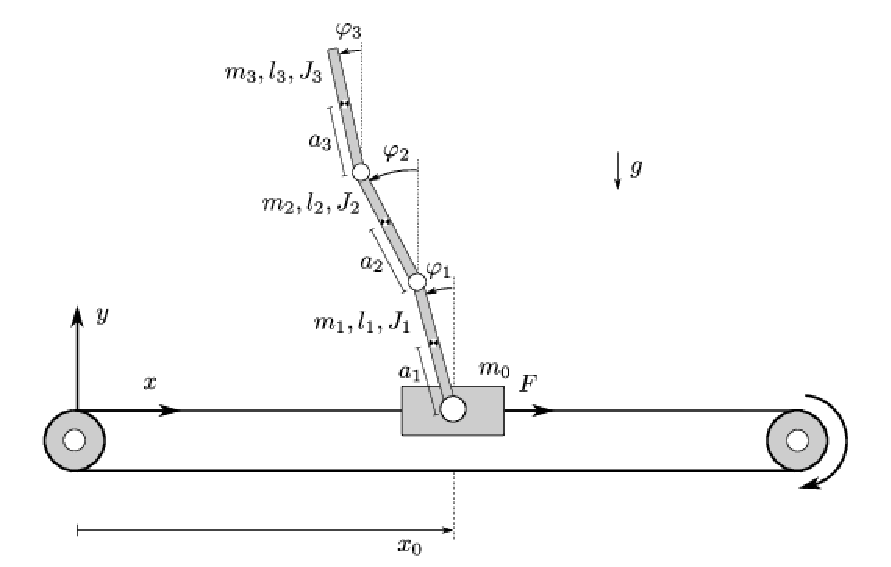
\includegraphics[width=90mm]{triple_pendulum.pdf}
		\caption{Triple Pendulum \\ \footnotesize{Source: Knoll, Carsten/Triple Pendulum on a Cart: Derivation of Equations of Motion and Simulation}}
	\end{figure}
	
	
	%%%%%%%%%%%%%%%%%%%%%% MDOEL EQUATIONS %%%%%%%%%%%%%%%%%%%%%%%%%%%
	
	\section{Model Equations} % MUST
	
	State Vector and Input Vector:
	\begin{align*}
		\underline{x} &= (p_1 \ p_2 \ p_3 \ q_1 \ \dot{p}_1 \ \dot{p}_2 \ \dot{p}_3 \ \dot{q}_1)^T &= (x_1 \ x_2 \ x_3 \ x_4 \ x_5 \ x_6 \ x_7 \ x_8)^T \\
		u &= F 
	\end{align*}
	
	\noindent Kinetic Energy:			
	\begin{subequations}
	\begin{align*}
		T &= \frac{1}{2}J_1x_5^2 + \frac{1}{2}J_2x_6^2 + \frac{1}{2}J_3x_7^2 + \frac{1}{2}m_0x_8^2 + \frac{1}{2}m_1(a_1^2x_5^2\sin x_1^2 + (-a_1x_5 \cos x_1 + x_8)^2) \\
		& + \frac{1}{2}m_2((-a_2x_6 \sin x_2 - l_1x_5 \sin x1 )^2 + (-a_2x_6 \cos x2 - l_1x_5 \cos x_1 + x_8)^2) \\
		& + \frac{1}{2}m_3((-a_2x_7 \sin x_3 - l_1x_5 \sin x_1 - l_2x_6 \sin x_2)^2 + (-a_2x_7 \cos x_3 - l_1x_5 \cos x_1 - l_2x_6 \cos x_2 + x_8)^2)
	\end{align*}
	\end{subequations}
	
	\noindent Potential Energy:			
	\begin{subequations}
	\begin{align*}
		V &= g(a_1m_1 \cos x1 + m_2(a_2 \cos x_2 + l_1 \cos x_1) + m_3(a_2 \cos x_3 + l_1 \cos x_1 + l_2 \cos x_2))
	\end{align*}
	\end{subequations}

	%%%%%%%%%%%%%%%%%%%%%% PARAMETERS | OUTPUTS %%%%%%%%%%%%%%%%%%%%%%%%%%%
	\noindent
	Parameters: $m_0, \, m_1, \, m_2, \, m_3, \, J_1, \, J_2, \, J_3, \, l_1, \, l_2, \, l_3, \, a_1, \, a_2, \, a_3, \, g$ % variables with constant, predefined value
	\\
	Outputs: \underline{x}
	
	
	%%%%%%%%%%%%%%%%%%%%%% EXEMPLARY PARAMETER VALUES %%%%%%%%%%%%%%%%%%%%%%%%%%%	
	
	\subsection{Exemplary parameter values}
	\begin{tabular}{cl}
\hline
  Symbol  & Value                                                                                                                                                                                \\
\hline
   $A$    & $\left[\begin{matrix}0.8189 & 0.0863 & 0.09 & 0.0813\\0.2524 & 1.0033 & 0.0313 & 0.2004\\-0.0545 & 0.0102 & 0.7901 & -0.258\\-0.1918 & -0.1034 & 0.1602 & 0.8604\end{matrix}\right]$ \\
   $B$    & $\left[\begin{matrix}0.0045 & 0.0044\\0.1001 & 0.01\\0.0003 & -0.0136\\-0.0051 & 0.0936\end{matrix}\right]$                                                                          \\
 $B_{1}$  & $\left[\begin{matrix}0.0045 & 0.0044\\0.1001 & 0.01\\0.0003 & -0.0136\\-0.0051 & 0.0936\end{matrix}\right]$                                                                          \\
 $C_{1}$  & $\left[\begin{matrix}1.0 & 0 & -1.0 & 0\\0 & 0 & 0 & 0\\0 & 0 & 0 & 0\end{matrix}\right]$                                                                                            \\
   $C$    & $\left[\begin{matrix}1.0 & 0 & 0 & 0\\0 & 0 & 1.0 & 0\end{matrix}\right]$                                                                                                            \\
 $D_{11}$ & $\left[\begin{matrix}0 & 0 & 0\\0 & 0 & 0\\0 & 0 & 0\end{matrix}\right]$                                                                                                             \\
 $D_{12}$ & $\left[\begin{matrix}0 & 0\\1.0 & 0\\0 & 1.0\end{matrix}\right]$                                                                                                                     \\
 $D_{21}$ & $\left[\begin{matrix}0 & 1.0 & 0\\0 & 0 & 1.0\end{matrix}\right]$                                                                                                                    \\
\hline
\end{tabular}

	%%%%%%%%%%%%%%%%%%%%%% DERIVATION & EXPLANATION %%%%%%%%%%%%%%%%%%%%%%%%%%%	
	
	\section{Derivation and Explanation} % SHOULD
	
	The Lagrangian mechanics was used for the solution.
	
	%%%%%%%%%%%%%%%%%%%%%% REFERENCES %%%%%%%%%%%%%%%%%%%%%%%%%%%
	
	\begin{thebibliography}{10}		
		\bibitem{But21}Knoll, Carsten: 
		\textit{Triple Pendulum on a Cart: Derivation of Equations of Motion and Simulation}, Jupyter Notebook published 2021. \\
		\url{https://github.com/cknoll/demo-material/blob/main/underactuated_systems/triple_pendulum_with_modeltools_plus_simulation-en.ipynb}
	\end{thebibliography}

\end{document}

